\documentclass[11pt]{article}
\usepackage[T1]{fontenc}
\usepackage{geometry, changepage}
\usepackage{amsmath, amssymb, amsthm, bm}
\usepackage{physics}
\usepackage{hyperref}
\usepackage{tikz}

\hypersetup{colorlinks=true, linkcolor=blue, urlcolor=cyan}
\setlength{\parindent}{0pt}
\setlength{\parskip}{5pt}

\newtheorem{theorem}{Theorem}
\newtheorem{lemma}{Lemma}
\newtheorem{claim}{Claim}
\newtheorem*{theorem*}{Theorem}
\newtheorem*{lemma*}{Lemma}
\newtheorem*{claim*}{Claim}

\renewcommand{\vec}[1]{\mathbf{#1}}
\newcommand{\uvec}[1]{\mathop{} \!\hat{\mathbf{#1}}}
\newcommand{\mat}[1]{\mathbf{#1}}
\newcommand{\tensor}[1]{\mathsf{#1}}

\renewcommand{\div}{\nabla \cdot}
\renewcommand{\curl}{\nabla \cross}
\renewcommand{\grad}{\nabla}
\renewcommand{\laplacian}{\nabla^{2}}

\title{MATH-UA 140: Assignment 1}
\author{James Pagan: September 2023}
\date{Professor Raquépas}

% --------------------------------------------- %

\begin{document}

\maketitle
\tableofcontents

% --------------------------------------------- %

\section{Problem 1}

\textbf{(a)} We have that 
\[
	\vec{u} \cdot  \vec{v} = \begin{bmatrix} 1 \\ 3 \\  2 \end{bmatrix} \cdot \begin{bmatrix} 2 \\ -1 \\ 1 \end{bmatrix} = 1(2) + 3(-1) + 2(1) = 1.
\]
\textbf{(b)} Let the angle between $\vec{u}$ and $\vec{v}$ be $\theta$; as the norms of $\vec{u}$ and $\vec{v}$ are nonzero,
\[
	\cos(\theta) = \frac{\vec{u} \cdot \vec{v}}{\norm{\vec{u}}\norm{\vec{v}}} = \frac{1}{\sqrt{1^{2} + 3^{2} + 2^{2}} \times \sqrt{2^{2} + (-1)^{2} + 1^{2}}} = \frac{1}{\sqrt{14} \times \sqrt{6}} = \frac{\sqrt{21}}{42}.
\]
Therefore, $\theta = \arccos(\frac{\sqrt{21}}{42}) \approx 1.46$ radians.

\textbf{(c)} No; observe that
\[
	\vec{u} + 3 \vec{v} = \begin{bmatrix} 1 \\ 3 \\ 2\end{bmatrix} + 3 \begin{bmatrix} 2 \\ -1 \\ 1 \end{bmatrix} = \begin{bmatrix} 1 \\ 3 \\ 2 \end{bmatrix} + \begin{bmatrix} 6 \\ -3 \\ 3 \end{bmatrix} = \begin{bmatrix} 7 \\ 0 \\ 5 \end{bmatrix} = \vec{w}.
\]
Therefore, the family $\{ \vec{u}, \vec{v}, \vec{w} \}$ is not independent.

% --------------------------------------------- %

\section{Problem 2}

\textbf{(a)} The span of $\vec{u}$ and $\vec{v}$ is a line,, pictured on the $xy$-plane below:

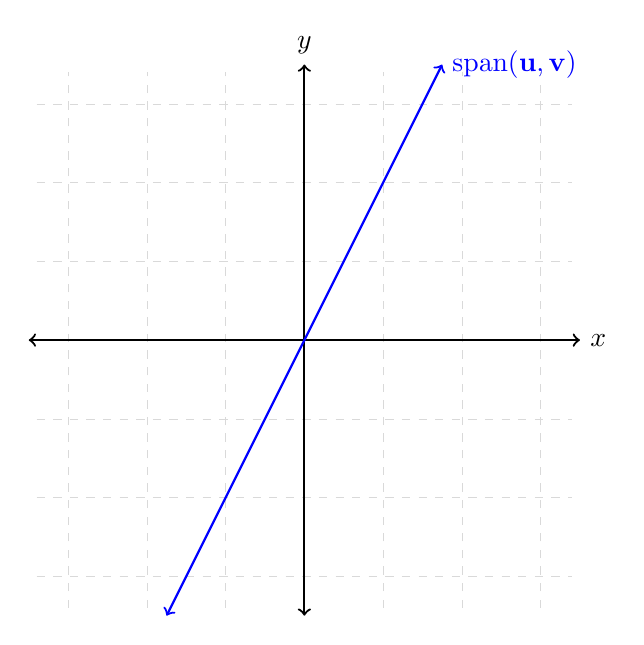
\begin{tikzpicture}
	\draw[help lines, color=gray!30, dashed] (-3.4,-3.4) grid (3.4,3.4);
	\draw[<->,thick] (-3.5,0)--(3.5,0) node[right]{$x$};
	\draw[<->,thick] (0,-3.5)--(0,3.5) node[above]{$y$};
	\draw[<->,thick, blue] (-1.75,-3.5)--(1.75,3.5) node[right]{$\operatorname{span} (\vec{u}, \vec{v})$};
\end{tikzpicture}

\textbf{(b)} The span of $\uvec{i}$ and $2\uvec{k}$ is the $zx$-plane, pictured in yellow in $\mathbb{R}^{3}$ as shown:

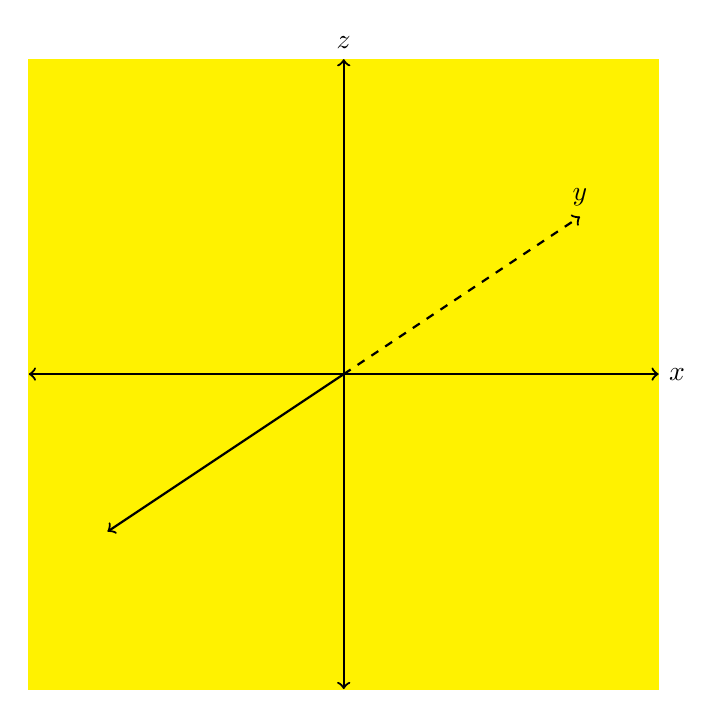
\begin{tikzpicture}
	\draw[help lines, color=gray!30, dashed] (-3.9,-3.9) grid (3.9,3.9);
	\filldraw[yellow] (-4,-4) rectangle (4, 4) node[anchor=west]{};
	\draw[<->,thick] (-4,0)--(4,0) node[right]{$x$};
	\draw[<->,thick] (0,-4)--(0,4) node[above]{$z$};
	\draw[<-,thick] (-3,-2)--(0,0) node[above]{};
	\draw[->,thick, dashed] (0, 0)--(3,2) node[above]{$y$};
\end{tikzpicture}

% --------------------------------------------- %

\section{Problem 3}

\textbf{(a)} True. If $\vec{w}$ is perpendicular to both $\vec{u}$ and $\vec{v}$, then $\vec{w} \cdot \vec{u} = \vec{w} \cdot \vec{v} = 0$. Therefore, 
\[
	\vec{w} \cdot (\vec{u} - \vec{v}) = \vec{w} \cdot \vec{u} - \vec{w} \cdot \vec{v} = 0 - 0 = 0,
\]
so $\vec{w}$ is perpendicular to $\vec{u} - \vec{v}$.

\textbf{(b)} False. The canonical basis vector $\uvec{i}$ is perpendicular to $\uvec{j}$ and $\uvec{k}$, but $\uvec{j}$ is not collinear with $\uvec{k}$.

\textbf{(c)} True. If $\vec{v} = \vec{0}$, then $\vec{v}$ is colinear with all vectors $\vec{w}$. Otherwise, observe that $\vec{u} \cdot \vec{v} = 0$ and $\vec{u}, \vec{v} \ne 0$ implies that $\vec{u}$ and $\vec{v}$ are linearly independent --- as $\mathbb{R}^{2}$ has dimension $2$, these two linearly independent vectors are a basis of $\mathbb{R}^{2}$.

Let $\lambda_{1}$ and $\lambda_{2}$ be constants such that $\lambda_{1} \vec{u} + \lambda_{2} \vec{v} = \vec{w}$. Then
\[
	0 = \vec{u} \cdot \vec{w} = \vec{u} \cdot (\lambda_{1} \vec{u} + \lambda_{2} \vec{v}) = \lambda_{1} (\vec{u} \cdot \vec{u}) + \lambda_{2} (\vec{u} \cdot \vec{v}) = \lambda_{1} \norm{\vec{u}}^{2}.
\]
However, $\norm{\vec{u}}^{2} \ne 0$ as $\vec{u} \ne \vec{0}$; then $\lambda_{1} = 0$. Then 
\[	
\vec{w} = \lambda_{1} \vec{u} + \lambda_{2} \vec{v} = 0 \vec{u} + \lambda_{2} \vec{v} = \lambda_{2} \vec{v};
\]
so $\vec{w}$ and $\vec{v}$ are collinear.

% --------------------------------------------- %

\section{Problem 4}

Using basic properties of the dot product, we have that
\begin{align*}
	\frac{\norm{\vec{u} + \vec{v}}^{2} - \norm{\vec{u} - \vec{v}}^{2}}{4} &= \frac{(\vec{u} + \vec{v}) \cdot (\vec{u} + \vec{v}) - (\vec{u} - \vec{v}) \cdot (\vec{u} - \vec{v})}{4} \\
	&= \frac{(\vec{u} \cdot \vec{u} + 2 (\vec{u} \cdot \vec{v}) + \vec{v} \cdot \vec{v}) - (\vec{u} \cdot \vec{u} - 2(\vec{u} \cdot \vec{v}) + \vec{v} \cdot \vec{v} )}{4} \\
	&= \frac{4(\vec{u} \cdot \vec{v})}{4} \\
	&= \vec{u} \cdot \vec{v}.
\end{align*}

% --------------------------------------------- %

\section{Problem 5}

\textbf{(a)} The form we desire is
\[
	\begin{bmatrix}
		1 & 2 \\ 0 & -1 \\ 4 & 3
		\end{bmatrix} \begin{bmatrix} x_{1} \\ x_{2} \end{bmatrix} = \begin{bmatrix} 2 \\ -3 \\ 8 \end{bmatrix}.
\]

\textbf{(b)} The form we desire is 
\[
	\begin{bmatrix} 1 & 1 & -1 \\ 2 & 0 & 1 \\ -1 & 3 & 0 \end{bmatrix} \begin{bmatrix} x_{1} \\ x_{2} \\ x_{3} \end{bmatrix} = \begin{bmatrix} 1 \\ 4 \\ 0 \end{bmatrix}.
\]

\section{Problem 6}

\textbf{(a)} As the former matrix is the identity matrix,
\[
\begin{bmatrix} 1 & 0 \\ 0 & 1 \end{bmatrix} \begin{bmatrix} a_{1, 1} & a_{1, 2} \\ a_{2, 1} & a_{2, 2} \end{bmatrix} = \begin{bmatrix} a_{1, 1} & a_{1, 2} \\ a_{2, 1} & a_{2, 2} \end{bmatrix}.
\]

\textbf{(b)} The matrix product we seek is
\[
	\begin{bmatrix}
		0 & 0 & 2 & 0 \\ 0 & 1 & 0 & 0 \\ 0 & 0 & 0 & 0 \end{bmatrix} \begin{bmatrix} 0 & 1 \\ 0 & 0 \\ -1 & 0 \\ 0 & 0  \end{bmatrix} = \begin{bmatrix} -2 & 0 \\ 0 & 0 \\ 0 & 0 \end{bmatrix}.
\]

\end{document}
